\documentclass[12pt,a4paper,titlepage,final]{report}
% \documentclass{report}

\usepackage[czech]{babel}
\usepackage[utf8]{inputenc}
\usepackage[T1, IL2]{fontenc}
\usepackage[scale=0.7,vmarginratio={1:2},heightrounded]{geometry}

\title{FYO - Fyzikální optika\\Wienerův pokus}
\author{Marek Salát, xsalat00}
\date{\today}

\usepackage[bookmarksopen,colorlinks,plainpages=false,urlcolor=blue]{hyperref}
\usepackage{url}

\usepackage{natbib}
\usepackage{graphicx}
\usepackage{epstopdf}
\usepackage{wrapfig}

\usepackage{lipsum}
\usepackage{xcolor}
\usepackage{caption}
\usepackage{subcaption}
\usepackage{listings}
\usepackage{verbatim}

\graphicspath{ {./figures/} }

\renewcommand{\thesection}{\arabic{section}}%
\newcommand\todo[1]{\textcolor{red}{#1}}

\begin{document}
\lstset{language=Matlab}

\maketitle

\pagestyle{plain}
\pagenumbering{roman}
\setcounter{page}{1}
\tableofcontents

\newpage
\begin{abstract}
Tato práce je zaměřena na Wienerův pokus. Je zde rozebrán život Otty Wienera a jeho příspěvků k experimentální fyzice.
Jsou zde rozebrány stojaté vlny. V tomto článku je velmi dopodrobna popsán Wienerův experiment, který dokazuje, že světlo je
tvořeno elektromagentickým vlněním a dokázal, že v chemických procesech při výrobě fotografii ma hlavní zásluhu
elektrická část světla. Součásti je také ukázková aplikace, která simuluje zadaný experiment.

\end{abstract}

\newpage
\pagestyle{plain}
\pagenumbering{arabic}
\setcounter{page}{1}

\section{Úvod}
Jméno Otty Wienera je často spojováno s pokusem, kterým dokázal existenci stojatých vlny. Nutno dodat, že okolo roku 1890, vědce velice poutala právě myšlenka stojatého vlnění. Zdálo se, že většina z nich tehdy nebyla přesvědčena o tom, že světlo je opravdu další 
forma elektromagnetického vlnění. Jednou z velkých překážek určitě byla velikost vln světla. Hertzovy radiové vlny dosahují vlnových délek v řádech metrů, zatímco vidítelné světlo má vlnové délky mezi tří sty až sedmi sty nanometry, což jsou miliardtiny metru. Takové to vzdálalenosti nemohou být pozorovány pouhým okem. Nebo mohou? Otto Wiener to díky svému nezměrnému důvtipu a vynalézavosti dokázal.

Určitě stojí za zmínku, že většina vědeckých článků té doby připouštěla (i v experimentech) v souladu s \emph{Mechanickou teorii světla} (teorie vyvrácena Albertem Einstainem v jeho teorii relativity), že světlo se šíří zatím neobjeveným prostředím zvaným \emph{éter}. Že je světlo
tvořeno elektromagnetickým vlněním, byla až dodatečná myšlenka v jeho práci.
 
Rok po Hetzově experimentu roku 1889, Otto Wiener provedl podobný experiment. Zjednodušeně řečeno vytvořil stojatou vlnu z monochromatického světla za pomocí stříbrné destičky a filmu. Přichozí vlna kolmá na zrcadlo mohla interferovat s vlnou odraženou, čímž vznikla stojatá vlna.
Aby tento jev zachytil, použi průhlený film, položený na destičce pod velice malým úhlem.

V tomto projektu se nejdříve podíváme na Wienerovu historii. Následně jsou zde rozebrány stojaté vlny, jako příprava pro rozbor Wienerova 
pokusu. Hlavní část této práce je věnována pokusu samotnému. Náplní projektu také  bylo vytvoření ukázkové aplikace, která je zde popsána
spolu s ovládáním a použitými technologemi. Aplikace simuluje Wienerův pokus, což znamená, že uživatel může vidět dění v simulačním čace s použitím animací.

\newpage 
 
\section{Otto Wiener}
% http://www.encyclopedia.com/doc/1G2-2830904649.html
% http://en.wikipedia.org/wiki/Otto_Wiener_%28physicist%29

Otto Wiener se narodil roku 1862 učiteli deskriptivní geometrie na Karlsruheské střední škole Christianu Wienerovi 
a matce Paulíně Hausrathové (sestra protestantského kněze). Wienerova matka zemřela na tyfus. Chlapec osiřel ve věku tří let. \cite{encyclopedia_otto}

\begin{figure}[!htb]
	\centering
	\begin{subfigure}[b]{0.4\textwidth}
 		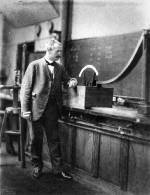
\includegraphics[width=\textwidth]{Otto_Wiener}
	\end{subfigure}
	~ %add desired spacing between images, e. g. ~, \quad, \qquad, \hfill etc.
      %(or a blank line to force the subfigure onto a new line)
	\begin{subfigure}[b]{0.4\textwidth}
 		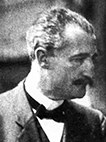
\includegraphics[width=\textwidth]{Otto_Wiener_mini}
	\end{subfigure}
	
	\caption{Otto Wiener, experimentální fyzik  vyfocen v Lipsku roku 1899.}\label{fig:otto}
\end{figure}       

Wiener studoval nejdříve v Karlsruhe, poté se přesunul do Berlína. Nakonec získal doktorát na Štrasburské univerzitě v roce 1887
pod vedením Augusta Kundta, za práci, která se zabívala změnou fáze (elektrické šložky) světla při odrazu. V roce 1890 se stal kvalifikovaným lektorem \uv{Stehende Lichtwellen} (stojaté vlny). Wiener je znám předevsím pro přínos v oblasti stojatých vln a také proto, že byl schopen změřit 
vlnovou délku světla (mimo jiné také šířku půhledného filmu). V roce 1895 byl povýšen a ve stejném roce (ve věku 32 let) se oženil s Linou Fennerovou. 
Roku 1895 Wiener přijal nabídku plného profesoriátu na Guessenské univerzitě. Jeho cílem zde bylo vybudovat nový institut fyziky. 
Zkušenosti z toho projektu využil v podobném projektu Lipské univerzity v roce 1899. \cite{encyclopedia_otto}

Jak bylo napsáno výše Wienerovo jméno je povětšinou spojováno s experimetny, které demonstrují stojaté vlny. V roce 1888 Heinrich Hertz
prokázal v Karlsruhelském institutu existenci elektromagnetických vln. Vlny, které detekoval, měly délku okolo osmi metrů. Rok později Wiener
provedl podobný experiment s elektromagnetickými vlnami světla, které jsou přibližně milionkrát menší než vlny, které detekoval Hertz. \cite{encyclopedia_otto}

Poté co obdržel doktorát, bylo jeho cílem změřit absobrci světla na tenké pruhledné kovové vrstvě. K provedení bylo zapotřebí znát šířku
vrstvy filmu a změnu fáze světla při reflekci (odrazu). Díky tomuto výzkumu se stal Wiener průkopníkem v této oblasti. \cite{encyclopedia_otto}

Stojaté vlny brzny nalezly uplatnení v Lippmannové barevné fotografii. Wiener měl také zálibu v technických problémech, především v letu ptáků, 
a byl velmi zaujat v leteckým průmyslem. Otto Wiener zemřel roku 1927 v neměckém Lipsku ve věku šedesáti čtyř let. \cite{wiki_otto}

\section{Stojaté vlny}
V roce 1890, byla myšlenka, že je světlo tvořeno elektromagnetickými
vlnami realtivně nová. J. C. Maxwell dokázal, že se elektromagnetické vlny šíří rychlostí světla. První člověk, který
byl toto schopen demonstrovat a dokázat existenci elektromagnetických vlny byl Heinrich Hertz. V roce 1887 dokázal, že jsou tyto vlny
konzistetní s Maxwellovou teorii, dokázal měřit jejich rychlost,
intenzitu elektrického pole a polarizaci. Dokonce se mu i 
podařilo vytvořti stojatou vlnu za pomocí zinkové destičky. \cite{skullsinthestars}

Stojatá vlna vznikne interferencí dvou vln, monochromatické vlny s vlnou odraženou od zrcadla, na kterou míříla kolmo.
Stojatá vlna pak osciluje nahoru a dolů bez zdálivého směru pohybu. Tento jev je znázorňuje následující serie obrázků.

\begin{figure}[!h]
        \centering
        \begin{subfigure}[b]{0.23\textwidth}
                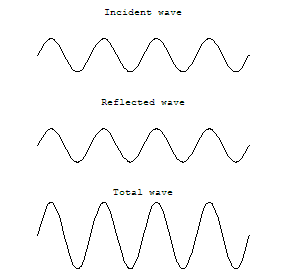
\includegraphics[width=\textwidth]{sin-1}
                \caption{}
                \label{fig:standing_wave:frame_1}
        \end{subfigure}%
        ~ %add desired spacing between images, e. g. ~, \quad, \qquad, \hfill etc.
          %(or a blank line to force the subfigure onto a new line)
        \begin{subfigure}[b]{0.23\textwidth}
                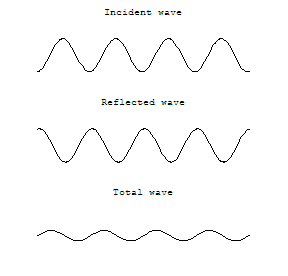
\includegraphics[width=\textwidth]{sin-2}
                \caption{}
                \label{fig:standing_wave:frame_2}
        \end{subfigure}
        ~ %add desired spacing between images, e. g. ~, \quad, \qquad, \hfill etc.
          %(or a blank line to force the subfigure onto a new line)
        \begin{subfigure}[b]{0.23\textwidth}
                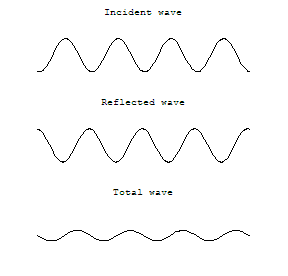
\includegraphics[width=\textwidth]{sin-3}
                \caption{}
                \label{fig:standing_wave:frame_3}
        \end{subfigure}
        ~ %add desired spacing between images, e. g. ~, \quad, \qquad, \hfill etc.
          %(or a blank line to force the subfigure onto a new line)
        \begin{subfigure}[b]{0.23\textwidth}
                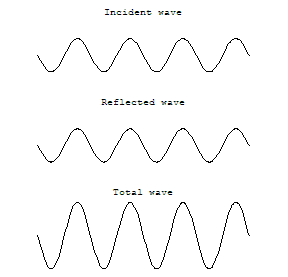
\includegraphics[width=\textwidth]{sin-4}
                \caption{}
                \label{fig:standing_wave:frame_4}
        \end{subfigure}
        \caption{Ukázka principu stojaté vlny. Pvní vlna směřuje zleva do prava, po odrazu změní fázi a směřuje zprav do leva (zobrazena jako druhá vlna). Výsledná stojatá vlna je vykreslena jako třetí.}\label{fig:standing_wave}
\end{figure}

Čtenář si může povšimnout, že u výsledné vlny jsou body, které neoscilují, stojí na místě, tyto body se nazývají uzly. Místa
kde vlná kmitá nejvíce, mezi minimem a maximem, říkamé kmity.
U viditelného světla je tato oscilace tak rychlá, že lidské oko
detekuje pouze průmernou světlost vlny. Světlo není tam, kde jsou uzly a místo se jeví jako tmavé, zatímco kmity se jeví jako světlé.
Na obrázku \ref{fig:intensityvsamplitude} je znázorněno jak by takovéto chování mohlo vypadat.

\begin{figure}[!htb]
   \centering
 	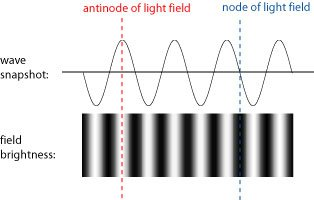
\includegraphics{intensityvsamplitude}
   \caption{Intenzita světla pro kmity a uzly. Kmity jsou světlá místa. Uzly jsou tmavá místa.}
   \label{fig:intensityvsamplitude}
\end{figure}

Jistě stojí za zmínku, že vzdálenost mezi uzly a kmity je 
právě polovina vlnové délky. Pozice uzlů a kmitů je určena tím
zda-li vlna po odrazu mení či nemění znaménko (fázi). Změna fáze je 
znázorněna na obrázku \ref{fig:eh_reflection}.

\begin{figure}[!htb]
   \centering
 	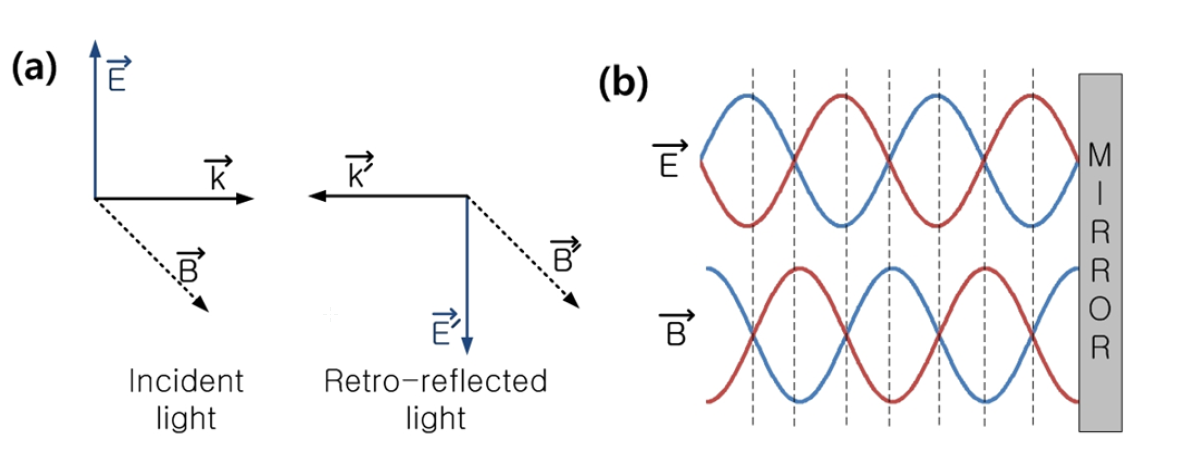
\includegraphics[width=\textwidth]{eh_reflection}
   \caption{Změna fáze světla při odrazu.}
   \label{fig:eh_reflection}
\end{figure}

Paprsek světla je tvořem dvěmi částmi. Jedná se o elektrickou složku
$E$ a magnetickou složku $H$. Obě tyto složky oscilují se stejnou
vlnovou dělkou, frekvencí a jsou ve fázi (viz obrázek \ref{fig:ehpropagation}), mohou také indukovat jak elektrické tak magnetické síly podle Lorentzova zákova sily. \citep{skullsinthestars}
\begin{equation}
F = e(E+\frac{v}{c}\times B)
\end{equation}

\begin{figure}[!htb]
   \centering
 	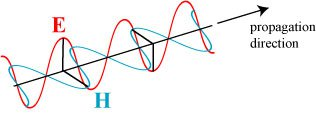
\includegraphics{ehpropagation}
   \caption{Propagace elektrické a magnetické části světla.}
   \label{fig:ehpropagation}
\end{figure}

V optice se můžeme setkat s tím, že u světla se znázorňuje pouze jeho
elektrická část. Také polarizace světla je určena podle směru elektrické složky. Magnetická složka je povětšinou ignorována.

\section{Wienerův pokus}
V roce 1890 nebyla úplně známá strutůra atomu a nebylo zcela zřejmé
jak svělo interaguje s hmotou. Hlavní otázkou bylo, zda-li
v chemických procesech při výrobě fotografii je spíše zapojeno 
$E$ nebo $H$. Jak se chová světlo pokud se odráží kolmo z povrchnu a jak to ovlivňuje fázi. 
Wiener, především inpirován Hertzem, doufal, že najde odpovědi na tyto otázky a pokud to bude možné,
demonstrovat stojaté vlnění. Jak již asi tušíte, Wiener uspěl. Separoval kmity, v intervalech přibližne $2\cdot 10^{n+1}$ $cm$ před
stříbrnou destičkou, vytvořené kolmo přicházejícím monochromatickým světlem. Wiener dokázal, že jsou to uzly, které leží
na povrchu zrcadla a né kmity. Odvodil tak, že při odrazu musí dojít ke změně fáze. Nezapomínaje, že tímto také dokázal, že právě
elektrická složka světla ma vliv na fotosensitivní vrstvu. Wienerův ohromující úspěch byl přijat a je dodnes považovát za mistrovské dílo
v experimentální fyzice.

Wiener navrhl následující pokus, popsán níže, za účelem objasnění role elektrického polevv optice. \ref{fig:energy_fig_wiener}

\begin{figure}[!htb]
   \centering
 	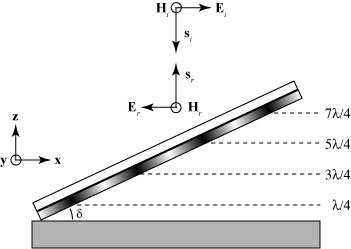
\includegraphics{energy_fig_wiener}
   \caption{Nákres Wienerova pokusu.}
   \label{fig:energy_fig_wiener}
\end{figure}

Monochromatická polorizovaná vlna směřuje kolmo na odrazovou plochu (stříbrná destička). V tomto
projektu předpokládáme dokonalé zrcadlo (z důvodu zachovaní jednoduchosti). Vlna mířící na zrcadlo společne s odraženo vlnou
vytvoří stojatou vlnu. Wiener použil tenky film (filmy by měl být výrazně tenčí než vlnová délka světla). 
Na filmu se mohly objevit dva vzory. Pokud se podívate na obrázek \ref{fig:energy_fig_wiener}, na výsledném filmu mohly být světlé a tmavé vertikální čáry, v případě, že film ovlivňuje elektrická část světla (to proto, že v prostoru z pohledu zhora, stejně jako na obrázku, se střídají světlé a tmavé proužky ve směru osy $z$). Pokud by se na filmu objevily 
horizontální světlé a tmavé proužky, znamenalo by to, že film byl ovlivněn magnetickou částí světla (to proto, že v prostoru z pohledu zhora, stejně jako na obrázku, se střídají světlé a tmavé proužky ve směru osy $y$). Pokud by byl film pod uhlem 0 (rovnoběžně se zrcadlem) nejenom, že by výsledek nešel vidět pouhym okem, ale také by byl film buď světlý nebo tmavý. Zde Wiener použil chytrý trik, při kterém film natočil o malý úhel. To způsobilo, že film nyní \emph{prořezává} světlé a tmavé vsrtvy, čimž dochází k pojekci intenzit stojaté vlny na film.

Na povrchu zrcadla, musí být elektrická část světla rovna nule, zatímco magnetická část zde nabýva svého maxima. Jednoduše se dá 
vypočíst, že maxima elektrické složky v ose $z$ budou
\begin{equation}
z = m\lambda / 4, \quad m=1,3,5,\ldots
\end{equation}
zatímco maxima magnetické složky se nachází
\begin{equation}
z = m\lambda / 4, \quad m=2,4,6,\ldots
\end{equation}

Kde $\lambda$ vyjadřuje vlnovou délku světla. Z rovnich vyplývá, že
maxima elektrické a magnetické složky se objevují v jiných bodech prostoru. Pozorováním filmu, může být pomocí světlých a tmavých proužků vyvozeno, zda-li má vliv elektrická nebo magnetická složka světla v chemických procesech při tvorbě fotografie.

Wiener tímto demonstroval, v souladu s elektromagnetickou teorii, že elektrická část světla je hlavní (důležitější) části.

Wiener měl před sebou ješte jednu překážku a tou byl film. Ten nejenom, že musel bý průhledný, aby mohlo světlo procházet zkrz, ale také musel být dostatečné tenký (významně tenčí než vlnová délka světla).
Wiener ve svém experimentu použil film, který byl asi 30x tenčí než 
vlnová delká světla které použival (sodiová oblouková lampa, přibližně s 600 $nm$). Film měl tehdy přibližne okolo 20 $nm$.

\section{Popis aplikace}
K demonstrování Wienerova pokusu jsem vytvořil aplikaci, která znázorňuje šíření elektrické části světelné vlny, simulace odrazu této vlny a 
součet obou vln (ukázka stojatého vlnění). Pohyb vln je animován. Na obrázku \ref{fig:aplikace} je příchozí vlna vycházející
ze droje světla (žlutá destička v levo) označena červeně. Odražená vlna od zrcadla (modrá destička v pravo) je zvýrazněna barvou červenou.
Výsledné stojaté vlně jsem přiřadil barvu fialovou. Nedílnou součásti je také film, na kterém je vykreslena aktuální intenzita světla.

\begin{figure}[!htb]
   \centering
 	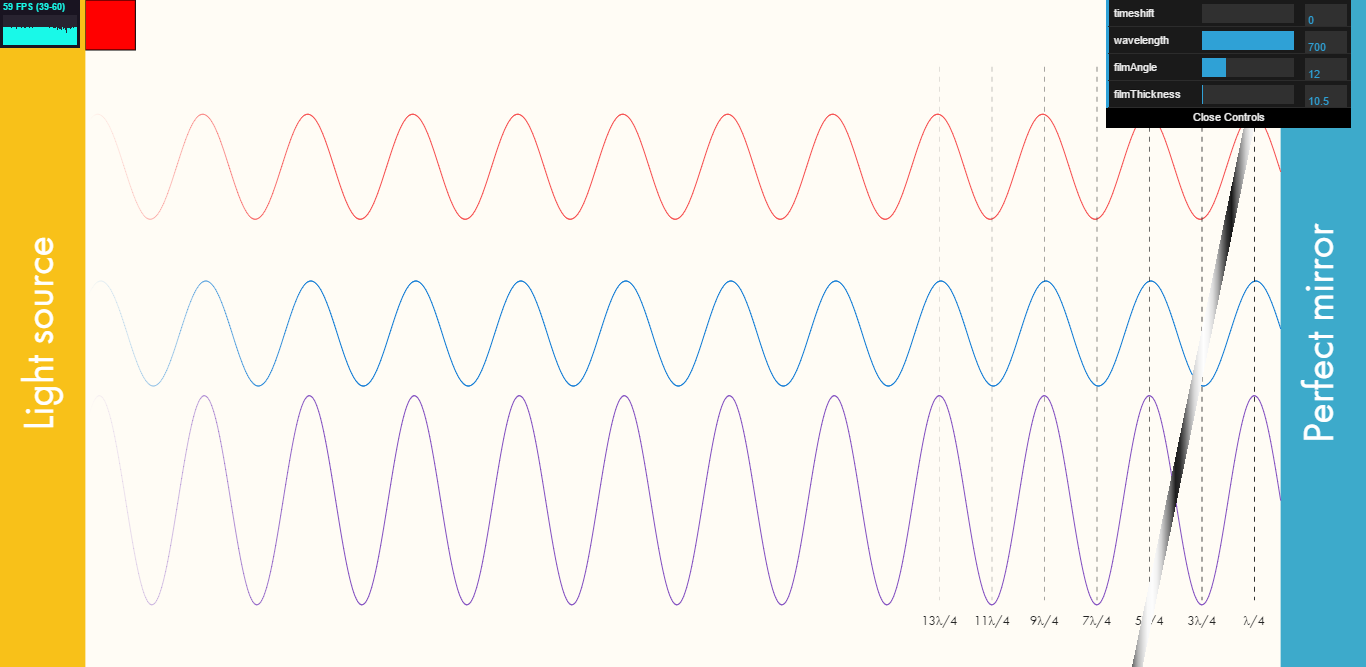
\includegraphics[width=\textwidth]{aplikace}
   \caption{Ukázka aplikace.}
   \label{fig:aplikace}
\end{figure}

V aplikace je možné nastavit rychlost simulace, případně simulaci úplně zastavit, pomocí \emph{timeshift}.
Dále může uživatel zvolit vlnovou délku světla pomocí \emph{wavelength}. Uživatel také vidí barvu zvoleného 
světla podle vlnové délky a to v levém horním rohu. Také je zde možnost nastavit 
úhel filmu (úhly jsou zámerně přechnané, v realném experimentu by byly okolo $0,001$ stupňů). A v nepolední řadě může uživatel
zvolit šírku filmu. Přerušované vertikální čáry označují místa maxim (kmitů) stojaté vlny v bodech.
\begin{equation}
z = m\lambda / 4, \quad m=1,3,5,\ldots
\end{equation}

Aplikace je napsána pomocí \emph{HTML5} a především pomocí prograovacího jazyka \emph{javascript}. K vykreslování
nebyly použity žádné externí knihovny a je použito výhradně nativní \emph{API} 2D \emph{context} a \emph{canvas}.
Celé zobrazení je responzivní (příspůsobuje se velikosti obrazovky). 

Nabídku ovládacích prvků je možné skrýt stiskem klávesy \emph{h}. Ovladací elementy byly vytvořeny knihovnou \emph{dat.gui}. Meření 
statistik zajišťuje knihovna \emph{stats}.

\section{Závěr}
V této práci byla rozebrána historie Otty Wienery. A to jak jeho důležitost pro experimentální fyziku tak i pro obyčejný život. 
Byl předveden důvtip zmiňovaného fyzika, který za svou práci v oblasti stojatých vln byl několikrát nominován na Nobelovu cenu. Byly zde rozebrány 
stojaté vlny a velice podrobně princip Wienerova pokusu. Představil jsem také webovou aplikaci, která čitelně znázorňuje a simuluje
Wienerův pokus.

Práce Otty Wienera je dokolanou ukázkou rčení \uv{\emph{V jednoduchosti je krása}}.

\textcolor{white}{
	\citep{wiki_otto}
	\citep{encyclopedia_otto}
	\cite{report}
	\citep{skullsinthestars}
}


\bibliographystyle{plain}
\bibliography{references}
\end{document}
